\chapter{Parameter Inference}
\label{ch:fastinference}

In this chapter\footnote{%
This chapter is based on \citet{maystre2015fast}.},
we study the problem of inferring parameters of models derived from Luce's choice axiom.
We begin by showing that the maximum-likelihood estimate (MLE) can be expressed as the stationary distribution of a Markov chain.
This conveys insight into several recently proposed spectral inference algorithms.
We then take advantage of this perspective and formulate a new spectral algorithm that generalizes and improves upon prior work.
With a simple adaptation, this algorithm can be used iteratively, producing a sequence of estimates that converges to the MLE.
The MLE version runs faster than competing approaches on a benchmark of five datasets.

%%%%%%%%%%%%%%%%%%%%%%%%%%%%%%%%
\section{Introduction}
\label{fi:sec:intro}

Markov chains have been used in recent work to aggregate inconsistent outcomes of pairwise comparisons and (partial) rankings \citep{dwork2001rank, negahban2012iterative, azari2013generalized}.
The idea is to build a Markov chain that is biased towards items that have won often, and to reduce the problem of ranking items to that of finding the \emph{stationary distribution} of the chain (the ranking is then induced by the items' stationary probabilities).
In this chapter, we highlight a connection between the MLE of models based on Luce's choice axiom and the stationary distribution of a Markov chain parametrized by the observed choices.
By formalizing this link, we unify previous algorithms and explicate them from an ML inference perspective.
Beyond this, the link suggests two new algorithms for parameter inference.
First, we develop a simple, consistent and computationally efficient spectral algorithm that is applicable to a wide range of models derived from Luce's choice axiom.
The exact formulation of the Markov chain used in the algorithm is distinct from related work \citep{negahban2012iterative, azari2013generalized} and achieves a significantly better statistical efficiency at no additional computational cost.
Second, we observe that with a small adjustment, the algorithm can be used iteratively, and it then converges to the MLE.
An evaluation on five real-world datasets reveals that it runs consistently faster than competing approaches and has a more predictable performance that does not depend on the structure of the data.
The key step, finding a stationary distribution, can be offloaded to commonly available linear-algebra primitives, which makes our algorithms  scale well.
The method we propose is intuitively pleasing, simple to understand and implement, and it outperforms the state of the art, hence we believe that it is highly useful to practitioners.

\paragraph{Outline of the Chapter}
We begin by introducing some notations and presenting a few useful facts about the MLE and about Markov chains.
In Section~\ref{fi:sec:relwork}, we discuss related work.
In Section~\ref{fi:sec:algorithms}, we present our algorithms, and in Section~\ref{fi:sec:experiments} we evaluate them on synthetic and real-world data.


\subsection{Maximum-Likelihood Estimate}
\label{fi:sec:mle}

%The log-likelihood \eqref{fi:eq:loglik} is not concave in $\bm{\gamma}$ (it can be made strictly concave using a simple reparametrization), but we briefly show in the supplementary material that it admits a unique stationary point, at the ML estimate $\bm{\gamma}^\star$.

Suppose that we collect $M$ independent choice observations in the multiset $\mathcal{D} = \{(c_m, \mathcal{A}_m) : m = 1, \ldots, M\}$.
Each observation consists of a choice $c_m$ among a set of alternatives $\mathcal{A}_m$;
we say that \emph{$i$ wins over $j$} and denote by $i \succ j$ whenever $i, j \in \mathcal{A}_m$ and $c_m = i$.
We postulate that the choices are generated from Luce's choice model, and for simplicity we denote the model parameter associated with item $c_m$ by $\gamma_m$.
From~\eqref{in:eq:luce}, it follows that the log-likelihood of parameters $\bm{\gamma}$ given observations $\mathcal{D}$ is given by
\begin{align}
\label{fi:eq:loglik}
\ell(\bm{\gamma}) = \sum_{m = 1}^M \bigg[ \log \gamma_m - \log{\sum_{j \in \mathcal{A}_m} \gamma_j} \bigg].
\end{align}
In order to ensure that the parameters are likelihood-identifiable, we assume without loss of generality that $\sum_i \gamma_i = 1$.
Next, we introduce a new object.

\begin{definition}[comparison graph]
The \emph{comparison graph} $\mathcal{G}_{\mathcal{D}} = (\mathcal{V}, \mathcal{E})$ is a directed graph with $\mathcal{V} = [N]$ and $(j, i) \in \mathcal{E}$ if and only if $i$ wins at least once over $j$ in $\mathcal{D}$.
\end{definition}

The existence and uniqueness of the MLE is completely determined by the connectivity of $\mathcal{G}_{\mathcal{D}}$, as the following well-known theorem shows.

\begin{theorem}[\citealp{zermelo1928berechnung, ford1957solution, hunter2004mm}]
\label{fi:thm:mlboth}
The likelihood function~\eqref{fi:eq:loglik} admits a unique maximizer $\bm{\gamma}^\star \in \mathbf{R}^N_{>0}$ such that $\sum_i \gamma^\star_i = 1$ if and only if $\mathcal{G}_{\mathcal{D}}$ is strongly connected.
\end{theorem}

Throughout this chapter, we will assume that $\mathcal{G}_{\mathcal{D}}$ is strongly connected.
In practice, if this assumption does not hold, we can consider each strongly-connected component separately.
Finally, note that even though $\ell(\bm{\gamma})$ admits a unique maximizer, it is not concave.
However, reparametrizing the model using $\theta_i \doteq \log \gamma_i$, the log-likelihood becomes
\begin{align*}
\ell(\bm{\theta}) = \sum_{m = 1}^M \bigg[ \theta_m - \log{\sum_{j \in \mathcal{A}_m} \exp \theta_j} \bigg],
\end{align*}
which is strictly concave in $\bm{\theta}$ (when $\mathcal{G}_{\mathcal{D}}$ is strongly connected).
Furthermore, for all $i \in [N]$,
\begin{align*}
\frac{\partial \ell}{\partial \gamma_i}
  = \frac{\partial \ell}{\partial \theta_i} \cdot \frac{\partial \theta_i}{\partial \gamma_i}
  = \frac{\partial \ell}{\partial \theta_i} \cdot \frac{1}{\gamma_i}
\quad \implies \quad
\frac{\partial \ell}{\partial \theta_i} = 0 \iff \frac{\partial \ell}{\partial \gamma_i} = 0.
\end{align*}
As the strictly concave function $\ell({\bm{\theta}})$ has a single stationary point, it follows that $\ell(\bm{\gamma})$ has a single stationary point at $\bm{\gamma}^\star$.


\subsection{Markov Chains}

We represent a finite, continuous-time Markov chain on $N$ states by a directed graph $\mathcal{G} = (\mathcal{V}, \mathcal{E})$, where $\mathcal{V} = [N]$ and $\mathcal{E}$ is the set of transitions with positive rate\footnote{%
Our exposition of Markov chains is succinct, and the interested reader is encouraged to consult \citet{levin2008markov} for a more thorough exposition.}.
If $\mathcal{G}$ is strongly connected, the Markov chain is said to be ergodic and admits a unique \emph{stationary distribution} $\bm{\pi} \in \mathbf{R}^N_{>0}$, $\sum_i \pi_i = 1$.
The \emph{global balance equations} relate the transition rates $\{ \lambda_{ij} \}$ to the stationary distribution as follows:
\begin{align}
\label{fi:eq:balance}
\sum_{j \ne i} \pi_i \lambda_{ij} = \sum_{j \ne i} \pi_j \lambda_{ji} \quad \forall i.
\end{align}
The stationary distribution is therefore invariant to changes in the time scale, i.e., to a rescaling of the transition rates.
Given transition rates $\bm{\Lambda} = [\lambda_{ij}]$, finding the stationary distribution $\bm{\pi}$ can be implemented in several different ways.
We distinguish implementations based on whether they consider a continuous-time or a discrete-time perspective on Markov chains.

\paragraph{Continuous-Time Perspective}
Let $\bm{Q}$ be the infinitesimal generator matrix of the Markov chain, i.e., $q_{ij} \doteq \lambda_{ij}$ and $q_{ii} \doteq - \sum_{j} \lambda_{ij}$.
The stationary distribution satisfies $\bm{\pi}^\Tr \bm{Q} = 0$; this is simply a matrix formulation of the global balance equations~\eqref{fi:eq:balance}.
Therefore, one approach to finding the steady-state distribution is to compute the rank-$1$ left nullspace of $\bm{Q}$.
This can be done, e.g., by LU decomposition, a basic linear-algebra primitive.
In the case where $\bm{Q}$ is dense, the running time of a typical implementation is $\BigO{N^3}$, but highly optimized parallel implementations such as that provided by LAPACK \citep{anderson1999lapack} are commonly available.
In the sparse case, LU decomposition can be done significantly faster using adapted algorithms, such as that of \citet{demmel1999supernodal}.

\paragraph{Discrete-Time Perspective}
Let $\epsilon < 1 / \max_i |q_{ii}|$, then $\bm{P} = \bm{I} + \epsilon \bm{Q}$ is the transition matrix of a discrete-time Markov chain that satisfies $\bm{\pi}^\Tr \bm{P} = \bm{\pi}$.
In this case, finding the steady-state distribution is equivalent to finding the left eigenvector associated to the leading eigenvalue of the transition matrix $\bm{P}$.
This is also a well-studied linear algebra problem for which plenty of efficient, off-the-shelf algorithms exist.
For example, power iteration methods can find the eigenvector in a few (sparse) matrix multiplications.
Beyond these well-known algorithms, recently-proposed randomized approaches such as that of \citet{halko2011finding} make it possible to scale to very large problem sizes ($N \sim 10^6$ or more).

Both the continuous-time and the discrete-time perspectives yield exactly the same resulting stationary distribution, and the algorithms presented in this paper are oblivious to this choice.

%%%%%%%%%%%%%%%%%%%%%%%%%%%%%%%%%%%%%%%%%%%%%%%%%%%%%%%%%%%%%%%%%%%%%%%%%
\section{Related Work}  %%%%%%%%%%%%%%%%%%%%%%%%%%%%%%%%%%%%%%%%%%%%%%%%%
\label{cr:sec:relwork}

A variant of the network choice model was recently introduced by \citet{kumar2015inverting}, in an article that lays much of the groundwork for this chapter.
Their generative model of traffic and the parametrization of transition probabilities based on Luce's axiom form the basis of our work.
\citeauthor{kumar2015inverting} define the \emph{steady-state inversion} problem as follows:
Given a graph $\mathcal{G}$ and a target stationary distribution, find transition probabilities that lead to the desired stationary distribution.
This problem formulation assumes that $\mathcal{G}$ satisfies restrictive structural properties (strong-connectedness, aperiodicity) and is valid only asymptotically, when the sequences of choices made by users are very long.
Our formulation is, in contrast, more general.
In particular, we eliminate any assumptions about the structure of $\mathcal{G}$ and cope with finite data in a principled way---in fact, our derivations are valid for choice sequences of any length.
One of our contributions is to explain the steady-state inversion problem in terms of (asymptotic) maximum-likelihood inference in the network choice model.
Furthermore, the statistical viewpoint that we develop also leads to
\begin{enuminline}
\item a robust regularization scheme, and
\item a simple and efficient EM-type inference algorithm.
\end{enuminline}
These important extensions make the model easier to apply to real-world data.

\paragraph{Luce's Choice Axiom}
The general problem of estimating parameters of models based on Luce's axiom has received considerable attention.
Several decades before Luce's seminal book \citep{luce1959individual}, \citet{zermelo1928berechnung} proposed a model and an algorithm that estimates the strengths of chess players based on pairwise comparison outcomes (his model would later be rediscovered by \citet{bradley1952rank}).
More recently, \citet{hunter2004mm} explained \citeauthor{zermelo1928berechnung}'s algorithm from the perspective of the minorization-maximization (MM) method.
This method is easily generalized to other models that are based on Luce's axiom, and it yields simple, provably convergent algorithms for maximum-likelihood (ML) or maximum-a-posteriori point estimates.
\citet{caron2012efficient} observe that these MM algorithms can be further recast as expectation-maximization (EM) algorithms by introducing suitable latent variables.
They use this observation to derive Gibbs samplers for a wide family of models.
We take advantage of this long line of work in Section~\ref{cr:sec:inference} when developing an inference algorithm for the network choice model.
In recent years, several authors have also analyzed the sample complexity of the ML estimate in Luce's choice model \citep{hajek2014minimax, vojnovic2016parameter} and investigated alternative spectral inference methods \citep{negahban2012iterative, azari2013generalized, maystre2015fast}.
Some of these results could be applied to our setting, but in general they require observing choices among well-identified sets of alternatives.
Finally, we note that models based on Luce's axiom have been successfully applied to problems ranging from ranking players based on game outcomes \citep{zermelo1928berechnung, elo1978rating} to understanding consumer behavior based on discrete choices \citep{mcfadden1973conditional}, and to discriminating among multiple classes based on the output of pairwise classifiers \citep{hastie1998classification}.

\paragraph{Network Analysis}
Understanding the preferences of users in networks is of significant interest in many domains.
For brevity, we focus on literature related to hyperlink graphs.
A method that has undoubtedly had a tremendous impact in this context is PageRank \citep{brin1998anatomy}.
PageRank computes a set of scores that are proportional to the amount of time a surfer, who clicks on links randomly and uniformly, spends at each node.
These scores are based only on the structure of the graph.
The network choice model presented in this chapter appears similar at first, but tackles a different problem.
In addition to the structure of the graph, it uses the traffic at each page, and computes a set of scores that reflect the (non-uniform) probability of clicking on each link.
Nevertheless, there are striking similarities in the implementation of the respective inference algorithms (see Section~\ref{cr:sec:experiments}).
The HOTness method proposed by \citet{tomlin2003new} is somewhat related, but tries to tackle a harder problem.
It attempts to estimate jointly the traffic and the probability of clicking on each link, by using a maximum-entropy approach.
At the other end of the spectrum, BrowseRank \citep{liu2008browserank} uses detailed data collected in users' browsers to improve on PageRank.
Our method uses only marginal traffic data that can be obtained without tracking users.
%In the context of mobility analysis, we mention that \citet{ashbrook2003using} and \citet{kafsi2015traveling}

%%%%%%%%%%%%%%%%%%%%%%%%%%%%%%%%
\section{Algorithms}
\label{fi:sec:algorithms}

We begin by expressing the MLE under the choice model as the stationary distribution of a Markov chain.
We then take advantage of this formulation to propose novel algorithms for model inference.
Although our derivation is made in the general choice model, we will also discuss implications for the special cases of pairwise data in Section~\ref{fi:sec:pairwise}, $K$-way ranking data in Section~\ref{fi:sec:partial}, and pairwise comparisons with ties in Section~\ref{fi:sec:ties}.

\subsection{MLE as a Stationary Distribution}

For each item $i \in [N]$, we define two sets of indices.
Let $\mathcal{W}_i \doteq \{ m : i \in \mathcal{A}_m, c_m = i \}$ and $\mathcal{L}_i \doteq \{ m : i \in \mathcal{A}_m, c_m \ne i \}$ be the indices of the observations where item $i$ wins over and loses against the alternatives, respectively.
We start from the log-likelihood $\ell(\bm{\gamma})$ in~\eqref{fi:eq:loglik};
the optimality condition $\nabla \ell = 0$ implies
\begin{align}
\left. \frac{\partial \ell(\bm{\gamma})}{\partial \gamma_i} \right\rvert_{\bm{\gamma} = \bm{\gamma}^\star}
    = \sum_{m \in W_i} \bigg[ \frac{1}{\gamma^\star_i} - \frac{1}{\sum_{j \in \mathcal{A}_m} \gamma^\star_j} \bigg]
      - \sum_{m \in \mathcal{L}_i} \frac{1}{\sum_{j \in \mathcal{A}_m} \gamma^\star_j} = 0 \quad \forall i \label{fi:eq:step1} \\
\iff  \sum_{j \ne i} \left[
    \sum_{m \in \mathcal{W}_i \cap \mathcal{L}_j} \frac{\gamma^\star_j}{\sum_{k \in \mathcal{A}_m} \gamma^\star_k}
    \;-\; \sum_{m \in \mathcal{W}_j \cap \mathcal{L}_i} \frac{\gamma^\star_i}{\sum_{k \in \mathcal{A}_m} \gamma^\star_k}
    \right] = 0 \quad \forall i. \label{fi:eq:mlbalance}
\end{align}
In order to go from \eqref{fi:eq:step1} to \eqref{fi:eq:mlbalance}, we multiply by $\gamma^\star_i$ and rearrange the terms.
To simplify the notation, let us further introduce the function
\begin{align*}
f(\mathcal{S}, \bm{\gamma}) \doteq \sum_{\mathcal{A} \in \mathcal{S}} \frac{1}{\sum_{i \in \mathcal{A}} \gamma_i},
\end{align*}
which takes observations $\mathcal{S} \subseteq \mathcal{D}$ and an instance of model parameters $\bm{\gamma}$, and returns a non-negative real number.
Let $\mathcal{D}_{i \succ j} \doteq \{ (c_m, \mathcal{A}_m) \in \mathcal{D} : m \in \mathcal{W}_i \cap \mathcal{L}_j \}$, i.e., the set of observations where $i$ wins over $j$.
Then \eqref{fi:eq:mlbalance} can be rewritten as
\begin{align}
\label{fi:eq:master}
\sum_{j \ne i} \gamma^\star_i \cdot f(\mathcal{D}_{j \succ i}, \bm{\gamma}^\star)
= \sum_{j \ne i} \gamma^\star_j \cdot f(\mathcal{D}_{i \succ j}, \bm{\gamma}^\star) \quad \forall i.
\end{align}
This formulation conveys a new viewpoint on the MLE.
It is easy to recognize the global balance equations \eqref{fi:eq:balance} of a Markov chain on $N$ states (representing the items), with transition rates $\lambda_{ji} = f(\mathcal{D}_{i \succ j}, \bm{\gamma}^\star)$ and stationary distribution $\bm{\gamma}^\star$.
These transition rates have an interesting interpretation: $f(\mathcal{D}_{i \succ j}, \bm{\gamma})$ is the count of how many times $i$ wins over $j$, weighted by the strength of the alternatives.
At this point, it is useful to observe that for any parameters $\bm{\gamma}$, $f(\mathcal{D}_{i \succ j}, \bm{\gamma}) > 0$ if and only if $(j,i) \in \mathcal{E}$.
Combined with the assumption that $\mathcal{G}$ is strongly connected, it follows that any $\bm{\gamma}$ parametrizes the transition rates of an ergodic (homogeneous) Markov chain.
The ergodicity of the inhomogeneous Markov chain, where the transition rates are constantly updated to reflect the current distribution over states, is shown by the following theorem.
\begin{theorem}
\label{fi:thm:convergence}
The Markov chain with inhomogeneous transition rates $\lambda_{ji} = f(\mathcal{D}_{i \succ j}, \bm{\gamma})$ converges to the maximum-likelihood estimate $\bm{\gamma}^\star$, for any initial distribution in the open probability simplex.
\end{theorem}

\begin{proof}[Proof]
Let $\bm{Q}(\bm{\gamma})$ be the infinitesimal generator matrix of the Markov chain $\bm{\gamma}(t)$.
The dynamics of the Markov chain are described by the differential equation
\begin{align}
\label{fi:eq:dynsys}
\frac{d \bm{\gamma}}{dt} = \bm{\gamma}^\Tr \bm{Q}(\bm{\gamma}).
\end{align}
By construction, the invariant distributions of the Markov chain coincide with the maximizers of the log-likelihood~\eqref{fi:eq:loglik}.
Hence, we know that $\bm{\gamma}^\star$ is the unique equilibrium point for~\eqref{fi:eq:dynsys}, i.e., satisfying $\bm{\gamma}^\Tr \bm{Q}(\bm{\gamma}) = \bm{0}$.
We will now show that this point is globally and asymptotically stable, i.e., $\bm{\gamma}(t) \to \bm{\gamma}^\star$ as $t \to \infty$ for any $\bm{\gamma}(0)$ in the open probability simplex.
To this end, it suffices to show that $V(\bm{\gamma}) = - \ell(\bm{\gamma}) + \ell(\bm{\gamma}^\star)$ is a Lyapunov function for the dynamical system~\eqref{fi:eq:dynsys}.
First, we have that $V(\bm{\gamma}^\star) = 0$ and $V(\bm{\gamma}) > 0$ for all $\bm{\gamma} \ne \bm{\gamma}^\star$ (by definition of the MLE).
Second, we note that $\bm{\gamma}^\Tr \bm{Q}(\bm{\gamma}) = \Diag{\bm{\gamma}} \nabla \ell(\bm{\gamma})$.
Hence,
\begin{align*}
\frac{dV}{dt}
    = \left( \nabla V \right)^\Tr \frac{d \bm{\gamma}}{dt}
    = - [\nabla \ell(\bm{\gamma})]^\Tr \Diag{\bm{\gamma}} \nabla \ell(\bm{\gamma})
    < 0,
\end{align*}
for all $\bm{\gamma} \ne \bm{\gamma}^\star$.
Third, $\ell(\bm{\gamma})$ grows unboundedly as $\bm{\gamma}$ approaches the boundary of the probability simplex \citep[Lemma~1]{hunter2004mm} and therefore $V(\bm{\gamma})$ does so as well.
The result then follows by applying the Barbashin-Krasovskii theorem, a standard result found, e.g., in \citet[Chapter~3]{khalil1996nonlinear}.
\end{proof}


\subsection{Approximate and Exact ML Inference}

We approximate the Markov chain described in \eqref{fi:eq:master} by considering a priori that all alternatives have equal strength.
That is, we set the transition rates $\lambda_{ji} \doteq f(\mathcal{D}_{i \succ j}, \bm{\gamma})$ by fixing $\bm{\gamma}$ to $[1/N \; \cdots \; 1/N]^\Tr$.
For $i \ne j$, the contribution of $i$ winning over $j$ to the rate of transition $\lambda_{ji}$ is $N / \Abs{\mathcal{A}}$.
In other words, for each observation, the winning item is rewarded by a fixed amount of incoming rate that is evenly split across the alternatives (the chunk allocated to itself is discarded).
We interpret the stationary distribution $\bar{\bm{\gamma}}$ as an estimate of model parameters.
Algorithm~\ref{fi:alg:lsr} summarizes this procedure, called \emph{Luce Spectral Ranking} (LSR).
%Note that as this Markov chain has different transition rates than that of \eqref{fi:eq:master}, $\bar{\bm{\gamma}} \ne \bm{\gamma}^\star$ in general.
If we consider a growing number of observations, LSR converges to the true model parameters $\bm{\gamma}'$, even in the restrictive case where the sets of alternatives are fixed.

\begin{algorithm}[t]
  \caption{Luce Spectral Ranking}
  \label{fi:alg:lsr}
  \begin{algorithmic}[1]
    \Require observations $\mathcal{D}$
    \State $\bm{\Lambda} \gets \bm{0}_{N \times N}$
    \For{$(i, \mathcal{A}) \in \mathcal{D}$}
      \For{$j \in \mathcal{A} \setminus \{ i \}$}
        \State $\lambda_{ji} \gets \lambda_{ji} + N / \Abs{\mathcal{A}}$
      \EndFor
    \EndFor
    \State \Return stationary distribution of Markov chain $\bm{\Lambda}$
  \end{algorithmic}
\end{algorithm}

\begin{theorem}
\label{fi:thm:consistency}
Let $\mathcal{U} = \{ \mathcal{A}_n \}$ be a collection of sets of alternatives such that for any partition of $\mathcal{U}$ into two non-empty sets $\mathcal{S}$ and $\mathcal{T}$, $\left( \cup_{\mathcal{A} \in \mathcal{S}} \mathcal{A} \right) \cap \left( \cup_{\mathcal{A} \in \mathcal{T}} \mathcal{A} \right) \ne \varnothing$.
Let $M_n$ be the number of choices observed over alternatives $\mathcal{A}_n$.
Then $\bar{\bm{\gamma}} \to \bm{\gamma}'$ as $M_n \to \infty \ \forall n$.
\end{theorem}

\begin{proof}
Let $M \to \infty$ be a shorthand for $M_n \to \infty \ \forall n$.
The condition on $\mathcal{U}$ is equivalent to stating that the hypergraph $H = (\mathcal{V}, \mathcal{U})$, with $\mathcal{V} = [N]$, is connected.
It implies that, asymptotically, the comparison graph $\mathcal{G}$ is strongly connected.
Indeed, for a given set of alternatives $\mathcal{A}_n$, let $i, j \in \mathcal{A}_n$.
The probability that $(j, i) \in \mathcal{E}$ is
\begin{align*}
1 - \left(1 - \frac{\gamma'_i}{\sum_{k \in \mathcal{A}_n} \gamma'_k} \right)^{M_n}
> 1 - (1 - \gamma'_i)^{M_n}
\xrightarrow{M_n \to \infty} 1,
\end{align*}
where we use the fact that $\gamma'_i > 0$ for all $i$.
Therefore, asymptotically, every alternative set $\mathcal{A}_n$ forms a clique in $\mathcal{G}$.
By assumption of connectivity on the hypergraph $\mathcal{H}$, the comparison graph $\mathcal{G}$ is strongly connected.

Now that we know that the Markov chain is asymptotically ergodic, we will show that the stationary distribution matches the true model parameters.
Let $c^n_m$ be a random variable denoting the item chosen in the $m$-th observation over alternatives $\mathcal{A}_n$, and let
$1\{\mathcal{X}\}$ be the indicator variable for the event $\mathcal{X}$.
By the law of large numbers, for any item $i \in \mathcal{A}_n$,
\begin{align}
\label{fi:eq:lln}
\lim_{M_n \to \infty} \frac{1}{M_n} \sum_{m = 1}^{M_n} 1\{c^n_m = i\} = \frac{\gamma'_i}{\sum_{k \in A_n} \gamma'_k}.
\end{align}
Now consider two items $i$ and $j$.
If they have never been compared, $\lambda_{ij} = \lambda_{ji} = 0$.
Otherwise, suppose that they have been compared in alternative sets whose indices are in $\mathcal{B} = \{ n : i, j \in \mathcal{A}_n \}$
By construction of the transition rates in LSR, we have that
\begin{align*}
\frac{\lambda_{ij}}{\lambda_{ji}}
= \frac{\sum_{n \in \mathcal{B}} \sum_{m = 1}^{M_n} 1\{c^n_m = j\} \ N / \Abs{\mathcal{A}_n}}
       {\sum_{n \in \mathcal{B}} \sum_{m = 1}^{M_n} 1\{c^n_m = i\} \ N / \Abs{\mathcal{A}_n}}.
\end{align*}
From \eqref{fi:eq:lln} it follows that
\begin{align*}
\lim_{M \to \infty}\frac{\lambda_{ij}}{\lambda_{ji}}
    = \frac{\sum_{n \in \mathcal{B}} (\gamma'_j / \sum_{k \in A_n} \gamma'_k) \ N / \Abs{\mathcal{A}_n}}
         {\sum_{n \in \mathcal{B}} (\gamma'_i / \sum_{k \in A_n} \gamma'_k) \ N / \Abs{\mathcal{A}_n}}
    = \frac{\gamma'_j }{\gamma'_i}.
\end{align*}
Therefore, when $M \to \infty$,
\begin{align*}
\sum_{j \ne i} \gamma'_i \lambda_{ij} = \sum_{j \ne i} \gamma'_i \left( \frac{\gamma'_j}{\gamma'_i} \lambda_{ji} \right)
                                    = \sum_{j \ne i} \gamma'_j \lambda_{ji}  \quad \forall i.
\end{align*}
It is easy to recognize the global balance equations, and it follows that $\bm{\gamma}'$ is the stationary distribution of the asymptotical Markov chain.
\end{proof}

Starting from the LSR estimate, we can iteratively refine the transition rates of the Markov chain and obtain a sequence of estimates.
By \eqref{fi:eq:master}, the only fixed point of this iteration is the MLE $\bm{\gamma}^\star$.
We call this procedure I-LSR and describe it in Algorithm~\ref{fi:alg:ilsr}.

%In Section~\ref{fi:sec:experiments}, we will investigate in detail the performance and practical advantages of this algorithm over the others for computing the ML estimate.
%For now, we will only note that because LSR is consistent implies that asymptotically, a single iteration is enough.
%This is in contrast to the MM algorithm \citep{hunter2004mm}, which is not consistent.

\begin{algorithm}[t]
  \caption{Iterative Luce Spectral Ranking}
  \label{fi:alg:ilsr}
  \begin{algorithmic}[1]
    \Require observations $\mathcal{D}$
    \State $\bm{\gamma} \gets [1/N \; \cdots \; 1/N]^\Tr$
    \Repeat
      \State $\bm{\Lambda} \gets \bm{0}_{N \times N}$
      \For{$(i, \mathcal{A}) \in \mathcal{D}$}
        \For{$j \in \mathcal{A} \setminus \{ i \}$}
          \State $\lambda_{ji} \gets \lambda_{ji} + 1 / \sum_{k \in \mathcal{A}} \gamma_k$
        \EndFor
      \EndFor
      \State $\bm{\gamma} \gets$ stationary distribution of Markov chain $\bm{\Lambda}$
    \Until{convergence}
  \end{algorithmic}
\end{algorithm}

LSR (or one iteration of I-LSR) entails 
\begin{enuminline}
\item filling a matrix of (weighted) pairwise counts and
\item finding a stationary distribution.
\end{enuminline}
Let $D \doteq \sum_{m} \Abs{\mathcal{A}_m}$, and let $S$ be the running time of finding the stationary distribution.
Then LSR has running time $\BigO{D + S}$.
As a comparison, one iteration of the MM algorithm \citep{hunter2004mm} is $\BigO{D}$.
Finding the stationary distribution can be implemented in different ways.
% with $S$ ranging from $\BigO{\min(D, N^2)}$ for power methods to $\BigO{N^3}$ for a dense LU decomposition.
For example, in a sparse regime where $D \ll N^2$, the stationary distribution can be found with the power method in a few $\BigO{D}$ sparse matrix multiplications.
In practice, whether $D$ or $S$ turns out to be dominant in the running time is not a foregone conclusion.

\subsection{Bradley--Terry Model}
\label{fi:sec:pairwise}

A widely-used special case of Luce's choice model occurs when all sets of alternatives contain exactly two items, i.e., when the data consists of pairwise comparisons.
This model was proposed by \citet{zermelo1928berechnung}, and later by \citet{bradley1952rank}.
As the stationary distribution is invariant to changes in the time-scale, we can rescale the transition rates and set $\lambda_{ji} \doteq |\mathcal{D}_{i \succ j}|$ when using LSR on pairwise data.
Let $\mathcal{S}$ be the set containing the pairs of items that have been compared at least once.
In the case where each pair $(i, j) \in \mathcal{S}$ has been compared exactly $C$ times, LSR is strictly equivalent to a continuous-time Markov-chain formulation of Rank Centrality \citep{negahban2012iterative}.
In fact, our derivation justifies Rank Centrality as an approximate ML inference algorithm for the Bradley--Terry model.
Furthermore, we provide a principled extension of Rank Centrality to the case where the number of comparisons observed is unbalanced.
Rank Centrality considers transition rates proportional to the \emph{ratio} of wins, whereas \eqref{fi:eq:master} justifies making transition rates proportional to the \emph{count} of wins.

\citet{negahban2012iterative} also provide an upper bound on the error rate of Rank Centrality, which essentially shows that it is minimax-optimal.
Because the two estimators are equivalent in the setting of balanced pairwise comparisons, the bound also applies to LSR.

\subsection{Plackett--Luce Model}
\label{fi:sec:partial}

Another case of interest is when observations do not consist of only a single choice, but of a ranking over the alternatives.
We now suppose $M$ observations consisting of $K$-way rankings, $2 \le K \le N$.
For conciseness, we suppose that $K$ is the same for all observations.
Let one such observation be $i(1) \succ \cdots \succ i(K)$, where $i(r)$ is the item with $r$-th rank.
The Plackett--Luce model (c.f. Section~\ref{in:sec:choice}) posits
\begin{align*}
\Prob{ i(1) \succ \cdots \succ i(K) }
  = \prod_{r = 1}^{K} \frac{\gamma_{i(r)}}{\sum_{s = r}^{K} \gamma_{i(s)}}.
\end{align*}
A ranking can thus be interpreted as a sequence of $K-1$ independent choices:
choose the first item, then choose the second among the remaining alternatives, etc.
With this point of view in mind, LSR and I-LSR can easily accommodate data consisting of $K$-way rankings, by decomposing the $M$ observations into $M' = M (K - 1)$ choices.

\citet{azari2013generalized} provide a class of consistent estimators for the Plackett--Luce model, using the idea of breaking rankings into pairwise comparisons.
Although they explain their algorithms from a generalized-method-of-moments perspective, it is straightforward to reinterpret their estimators as stationary distributions of particular Markov chains.
In fact, for $K = 2$, their algorithm GMM-F is identical to LSR.
When $K > 2$ however, breaking a ranking into $\binom{K}{2}$ pairwise comparisons implicitly makes the (incorrect) assumption that these comparisons are statistically independent.
The Markov chain that LSR builds breaks rankings into pairwise rate contributions, but weights the contributions differently depending on the rank of the winning item.
In Section~\ref{fi:sec:experiments}, we show that this weighting turns out to be crucial.
Our approach yields a significant improvement in statistical efficiency, yet keeps the same attractive computational cost and ease of use.


\subsection{Rao--Kupper Model}
\label{fi:sec:ties}

The link between the MLE and the stationary distribution of a Markov chain seemingly applies to other variants and extensions of Luce's choice model.
As an illustration, we consider the model proposed by \citet{rao1967ties}, which extends the Bradley--Terry model to the case where a comparison between two items can result in a tie.
This model is useful, e.g., for chess, where a significant fraction of comparison outcomes do not result in either a win or a loss.
Letting $\alpha \in [1, \infty)$, the probabilities of $i$ winning over and tying with $j$, respectively, are given by
\begin{align*}
p(i \succ j) &= \frac{\gamma_i}{\gamma_i + \alpha \gamma_j}, \\
p(i \equiv j) &= \frac{\gamma_i \gamma_j(\alpha^2 - 1)}{(\gamma_i + \alpha\gamma_j)(\alpha \gamma_i + \gamma_j)}.
\end{align*}
Informally, the parameter $\alpha$ controls the expected probability of observing a tie in the comparison of two items of equal strength.
We assume that $\alpha$ is fixed, and derive an expression of the MLE $\bm{\gamma}^\star$.
Let $a_{ji}$ be the number of times $i$ wins over $j$, and $t_{ij} = t_{ji}$ be the number of ties between $i$ and $j$.
The log-likelihood can be written as
\begin{align*}
\ell(\bm{\gamma}) &=
  \sum_i \sum_{j \ne i}
  a_{ji} \left[ \log \gamma_i - \log(\gamma_i + \alpha \gamma_j) \right] \\
    &+ \sum_i \sum_{j > i}
    t_{ij} \left[ \log \gamma_i + \log \gamma_j  + \log(\alpha^2 - 1)
     - \log(\gamma_i + \alpha \gamma_j) - \log(\alpha \gamma_i + \gamma_j) \right].
\end{align*}
This function admits a unique MLE $\bm{\gamma}^\star$, and the optimality condition $\nabla \ell = 0$ implies
\begin{align*}
\left. \frac{\partial \ell(\bm{\gamma})}{\partial \gamma_i} \right\rvert_{\bm{\gamma}= \bm{\gamma}^\star}
    = &\sum_{j \ne i} \Bigg[ a_{ji} \bigg( \frac{1}{\gamma^\star_i} - \frac{1}{\gamma^\star_i + \alpha \gamma^\star_j} \bigg)
      - a_{ij} \frac{\alpha}{\alpha \gamma^\star_i + \gamma^\star_j} \\
      & \qquad {} + t_{ij} \bigg( \frac{1}{\gamma^\star_i} - \frac{1}{\gamma^\star_i + \alpha \gamma^\star_j} - \frac{\alpha}{\alpha \gamma^\star_i + \gamma^\star_j} \bigg) \Bigg] = 0 \\
    \iff & \sum_{j \ne i} \Bigg[ a_{ji} \frac{\alpha \gamma^\star_j}{\gamma^\star_i + \alpha \gamma^\star_j}
      - a_{ij} \frac{\alpha \gamma^\star_i}{\alpha \gamma^\star_i + \gamma^\star_j}
      + t_{ij} \frac{\alpha (\gamma^\star_j)^2 - \alpha (\gamma^\star_i)^2}{(\gamma^\star_i + \alpha \gamma^\star_j)(\alpha \gamma^\star_i + \gamma^\star_j)} \Bigg] = 0 \\
    \iff & \sum_{j \ne i} \Bigg[ \frac{a_{ji} + t_{ji}\tfrac{\gamma^\star_j}{\alpha \gamma^\star_i + \gamma^\star_j}}{\gamma^\star_i + \alpha \gamma^\star_j} \gamma^\star_j
      \; - \; \frac{a_{ij} + t_{ij}\tfrac{\gamma^\star_i}{\gamma^\star_i + \alpha \gamma^\star_j}}{\alpha \gamma^\star_i + \gamma^\star_j} \gamma^\star_i \Bigg] = 0.
\end{align*}
Therefore, the MLE can be interpreted as the stationary distribution of a Markov chain with transition rates
\begin{align*}
\lambda_{ij} = \frac{a_{ij} + t_{ij}\tfrac{\gamma^\star_i}{\gamma^\star_i + \alpha \gamma^\star_j}}{\alpha \gamma^\star_i + \gamma^\star_j}.
\end{align*}
Given these transition rates, the extension of Algorithms~\ref{fi:alg:lsr} and~\ref{fi:alg:ilsr} is straightforward.
For example, for LSR, the transition rates simplify to $\lambda_{ij} \propto a_{ij} + t_{ij} (1 + \alpha)^{-1}$.

Beyond the Rao--Kupper model, we believe that our algorithms can be generalized to further models that are based on the choice axiom.
However, this axiom is key, and other choice models (such as Thurstone's \citeyearpar{thurstone1927law}) do not seem to admit the stationary-distribution interpretation we derive here.

%%%%%%%%%%%%%%%%%%%%%%%%%%%%%%%%%%%%%%%%%%%%%%%%%%%%%%%%%%%%%%%%%%%%%%%%%
\section{Experimental Evaluation}  %%%%%%%%%%%%%%%%%%%%%%%%%%%%%%%%%%%%%%
\label{rs:sec:experiments}

In practice, the comparison budget for estimating a ranking from noisy data might typically be larger than that for a single call to Quicksort, and it might not exactly match the number of comparisons required to run a given number of calls to Quicksort to completion.
Building upon the observations made at the end of Section~\ref{rs:sec:poisson}, we suggest the following practical active-learning strategy:
for a budget of $M$ pairwise comparisons, run the sorting procedure repeatedly until the budget is depleted (the last call might have to be truncated).
Then, retain only the set of $M$ comparison pairs and their outcomes and discard the rankings produced by the sorting procedure.
The final ranking estimate is then induced from the MLE over the set of $M$ comparison outcomes.

In this section, we demonstrate the effectiveness of this sampling strategy on synthetic and real-world data.
In particular, we show that it is comparable to existing AL strategies at a minuscule fraction of the computational cost.


%%%%%%%%%%%%%%%%%%%%%%%%%%%%%%%%%%%%%%%%%%%%%%%%%%%%%%%%%%%%%%%%%%%%%%%%%
\subsection{Competing Sampling Strategies}

To assess the relative merits of our sorting-based strategy, we consider three strategies that we believe are representative of the state of the art in active preference learning.

\paragraph{Uncertainty Sampling}
Developed in the context of classification tasks, this popular active-learning heuristic suggests to greedily sample the point that lies closest to the decision boundary \citep{settles2012active}.
In the context of a ranking task, this corresponds to sampling the pair of items whose relative order is most uncertain.
After $t$ observations, given an estimate of model parameters $\bm{\theta}^t$, the strategy selects the $(t\!+\!1)$-st pair uniformly at random in
\begin{align*}
\Argmin_{i \ne j} \Abs{\theta^t_i - \theta^t_j}.
\end{align*}
This set can be computed in time \BigO{N \log N} by sorting the parameters.
The parameters themselves need to be estimated, e.g., using (penalized) ML inference that in practice can be the dominating cost.

\paragraph{Bayesian Methods}
If we have access to a full posterior distribution $q^t(\bm{\theta})$ instead of a point estimate $\bm{\theta}^t$, we can take advantage of the extra information on the uncertainty of the parameters to improve the selection strategy.
A principled approach to AL consists of sampling the point that maximizes the expected information gain \citep{mackay1992bayesian}.
That is, the pair of items at iteration $t+1$ is selected in
\begin{align}
\label{rs:eq:entreduc}
\Argmax_{i \ne j} H(q^t) - \Exp{H(q^{t+1})},
\end{align}
where $H(\cdot)$ denotes the entropy function.
A conceptually similar but slightly different selection strategy is given by \citet{chen2013pairwise}.
Letting $q_{ij}$ be the marginal distribution of $(\theta_i, \theta_j)$, the pair is selected in
\begin{align}
\label{rs:eq:kldiv}
\Argmax_{i \ne j} \Exp{ \KL(q^{t+1}_{ij} \Vert q^t_{ij}) },
\end{align}
where $\KL(\cdot)$ denotes the Kullback--Leibler divergence.
Computing the exact posterior is not analytically tractable for the BT model, but a Gaussian approximation can be found in time \BigO{N^3}.
Criteria \eqref{rs:eq:entreduc} and \eqref{rs:eq:kldiv} can be computed in constant time for each pair of items.
The dominating cost is again that of estimating $\bm{\theta}$ (or, in this case, $q(\bm{\theta})$).

In addition to these existing AL strategies, we also include in our experiments a variation of our sorting-based strategy that uses Mergesort instead of Quicksort.
In the noiseless setting, Mergesort is known to use on average $\approx \num{39}~\%$ fewer comparisons than Quicksort per run \citep{knuth1998art}, but it does not benefit from the theoretical guarantees developed in Section~\ref{rs:sec:theory}.


%%%%%%%%%%%%%%%%%%%%%%%%%%%%%%%%%%%%%%%%%%%%%%%%%%%%%%%%%%%%%%%%%%%%%%%%%
\subsection{Running Time}

In this section, we briefly discuss the running time of the methods.
We implement ML and Bayesian approximate inference algorithms for the BT model as a Python library\footnote{See: \url{http://lucas.maystre.ch/choix}.}.
For approximate Bayesian inference, we use a variant of the expectation-propagation algorithm outlined by \citet{chu2005extensions}.
All experiments are performed on a server with a \num{12}-core Xeon X5670 processor running at \num{2.93}~GHz.
Numerical computations take advantage of the Intel Math Kernel Library.

We illustrate the running time of AL strategies as follows.
For $N \in \{10^2, 10^3, 10^4 \}$, we generate outcomes for $N$ comparisons pairs chosen uniformly at random among $N$ items.
For each strategy, we then measure the time it takes to select the $(N\!+\!1)$-st pair of items adaptively.
The results are presented in Table~\ref{rs:tab:runningtime}.
Note that these numbers are intended to be considered as orders of magnitude, rather than exact values, as they depend on the particular combination of software and hardware that we use.
The running time of the Bayesian AL strategies exceed \num{10} hours for $N = 10^4$ and the calls were stopped ahead of completion.
Our sorting-based methods, like random sampling, are the only AL strategies whose running time is constant for increasing $N$ (and for increasing $M$).
In fact, their running time is negligible in comparison to the other strategies, including uncertainty sampling.

\begin{table}[t]
  \caption{
Time (in seconds) to select the $(N\!+\!1)$-st pair.
Values indicated by $\varepsilon$ are below $10^{-5}$.
See text for details.
}
  \label{rs:tab:runningtime}
  \centering
  \begin{tabular}{l ccc}
    \toprule
                  & \multicolumn{3}{c}{$T$ [s]} \\
                    \cmidrule(l){2-4}
    Strategy      & $N = 10^2$      & $N = 10^3$       & $N = 10^4$ \\
    \midrule
    uncertainty   & \num{0.05}      & \num{0.5}        & \num{11}      \\
    entropy       & \num{0.3}       & \num{40}         & ---           \\
    KL-divergence & \num{0.9}       & \num{71}         & ---           \\
    Mergesort     & $\varepsilon$   & $\varepsilon$    & $\varepsilon$ \\
    Quicksort     & $\varepsilon$   & $\varepsilon$    & $\varepsilon$ \\
    random        & $\varepsilon$   & $\varepsilon$    & $\varepsilon$ \\
    \bottomrule
  \end{tabular}
\end{table}


%%%%%%%%%%%%%%%%%%%%%%%%%%%%%%%%%%%%%%%%%%%%%%%%%%%%%%%%%%%%%%%%%%%%%%%%%
\subsection{Data Efficiency}

We now investigate three datasets and measure the displacement of rankings estimated from adaptively-chosen samples, as a function of the budget $M$.
Note that in order to use uncertainty sampling and Bayesian methods, it is necessary to choose a regularization strength or prior variance in the inference step.
Different values can result in drastically different outcomes (in particular for uncertainty sampling) and, in practice, choosing a good value can be a significant challenge\footnote{Observe that our sorting-based approach is entirely parameter-free and is therefore not affected by this issue.}.
In the following, we report results for the values that worked best \emph{a posteriori}.


\paragraph{Synthetic Dataset}

We generate $N$ i.i.d. parameters $\theta_1, \ldots, \theta_n$ uniformly in $[0, (N\!+\!1) / \lambda]$ and draw samples from $\BT(\bm{\theta})$.
The ground-truth ranking is the one induced by the parameters.
Figure~\ref{rs:fig:synthetic} presents results for $N = \num{200}$ and $\lambda = \num{5}$.
In comparison to random sampling, AL is very effective and results in significantly better ranking estimates for any given number of comparisons.
The two Bayesian methods, though being the most computationally expensive, perform the best for all values of $M$, but are nearly indistinguishable from uncertainty sampling.
The two sorting-based strategies perform similarly (with a small edge for Mergesort).
They are slightly worse than the Bayesian methods but are still able to reap most of the benefits of active learning.

\begin{figure}[t]
\centering
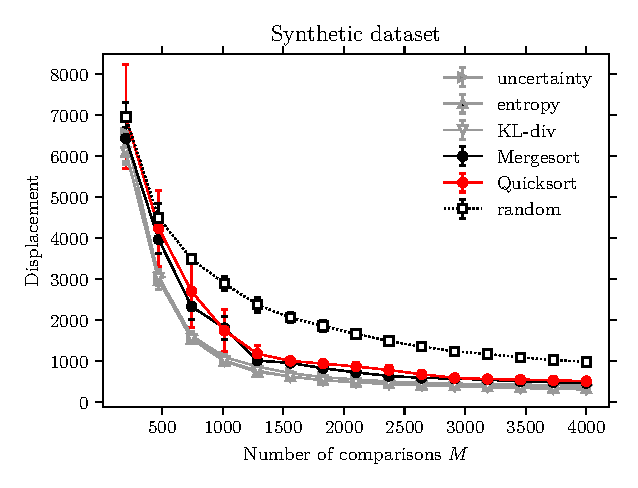
\includegraphics{rs-synthetic}
\caption{
Synthetic dataset with $\lambda = 5$ and $N = 200$.
The experiment is repeated \num{10} times, and we report the mean and the standard deviation.
Compared to random sampling, AL results in significantly better rankings for a given budget $M$.
}
\label{rs:fig:synthetic}
\end{figure}


\paragraph{Sushi Dataset}

\begin{figure}[t]
\centering
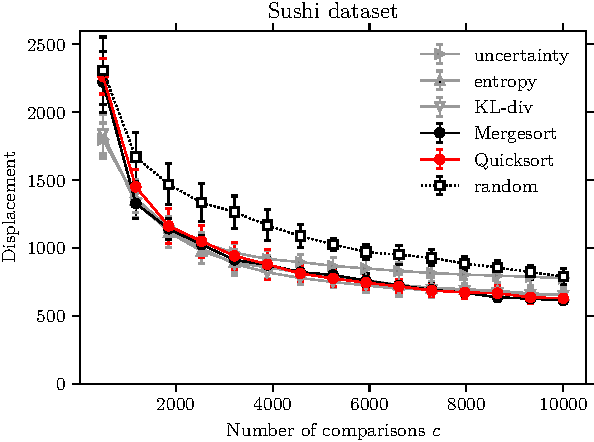
\includegraphics{rs-sushi}
\caption{
Results on two real-world datasets.
Every experiment is repeated \num{10} times, and we report the mean and the standard deviation.
Left: on the sushi dataset, sorting-based and Bayesian AL strategies have near-identical performance starting from $M \approx \num{1000}$.
Right: on the GIFGIF dataset, most AL strategies are computationally too expensive---except for sorting-based methods.
}
\label{rs:fig:sushi}
\end{figure}

Next, we consider a dataset of Sushi preferences \citep{kamishima2009efficient}.
In this dataset, \num{5000} respondents give a strict ordering over \num{10} different types of sushi.
These \num{10} sushi are chosen among a larger set of $N = \num{100}$ items.
To suit our purposes, we decompose each $10$-way partial ranking into pairwise comparisons, resulting in \num{225000} comparison outcomes.
We use all comparisons to fit a BT model that induces a ground-truth ranking\footnote{
The BT-induced ranking is almost the same as that obtained using the Copeland score.
The results are very similar if the Copeland aggregation is used as ground truth.}.

The comparisons are dense, and there is at least one comparison outcome for almost all pairs.
When an outcome for pair $(i,j)$ is requested, we sample uniformly at random over all outcomes observed for this pair.
In the rare case where no outcome is available, we return $i \prec j$ with probability $1/2$.
This enables us to compare sampling strategies in a realistic setting, where the assumptions of the BT model do not necessarily hold anymore.

Results are shown in Figure~\ref{rs:fig:sushi}.
Once again, active learning performs noticeably better than random sampling.
On this real-world dataset, the performance of our sorting-based strategies is indistinguishable from that of the Bayesian methods, after completing one entire call to the sorting procedure (slightly less than \num{1000} comparisons).
This result should be interpreted in light of the time needed to select all $10^4$ pairs: a fraction of a second for sorting-based strategies, and several hours for the Bayesian methods.
Finally, we observe that the performance of uncertainty sampling progressively degrades as $M$ increases.
A detailed analysis reveals that uncertainty sampling increasingly focuses on a small set of hard-to-discriminate pairs, symptomatic of a well-known issue \citep{settles2012active}.


\paragraph{GIFGIF Dataset}

\begin{figure}[t]
\centering
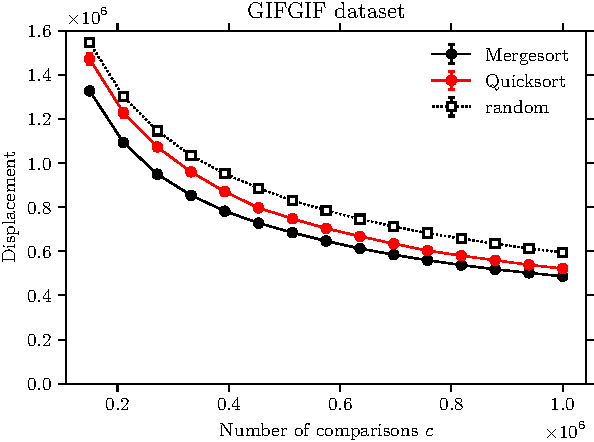
\includegraphics{rs-gifgif}
\caption{
Results on two real-world datasets.
Every experiment is repeated \num{10} times, and we report the mean and the standard deviation.
Left: on the sushi dataset, sorting-based and Bayesian AL strategies have near-identical performance starting from $M \approx \num{1000}$.
Right: on the GIFGIF dataset, most AL strategies are computationally too expensive---except for sorting-based methods.
}
\label{rs:fig:gifgif}
\end{figure}

GIFGIF\footnote{See \url{http://www.gif.gf/}.
Data available at \url{http://lucas.maystre.ch/gifgif-data}.} is a project of the MIT Media Lab that aims at explaining the emotions communicated by a collection of animated GIF images.
Users of the website are shown a prompt with two images and a question, ``Which better expresses $x$?'' where $x$ is one of 17 emotions.
The users can click on either image, or use a third option, \emph{neither}.
To date, over three million comparison outcomes have been collected.
For the purpose of our experiment, we restrict ourselves to a single emotion, \emph{happiness}; and we ignore outcomes that resulted in \emph{neither}.
We consider \num{106887} comparison outcomes over $N = \num{6120}$ items---a significant increase in scale compared to the Sushi dataset.

As the data, despite a relatively large number of comparisons, remains sparse (less than 20 comparisons per item on average), we proceed as follows.
We fit a BT model by using all the available comparisons and use the induced ranking as ground truth.
We then generate new, synthetic comparison outcomes from the BT model.
In this sense, the experiment enables us to compare sampling strategies by using a large BT model with realistic parameters.
The large number of items makes uncertainty sampling and the two Bayesian methods prohibitively expensive.
We try a simplified, computationally less expensive version of uncertainty sampling where, at every iteration, each item is compared to its two closest neighbors, but this heuristic fails spectacularly: The resulting displacement is over $5\times$ larger than random sampling for $M = 10^6$, and is therefore not reported here.

Figure~\ref{rs:fig:gifgif} compares the displacement of random sampling to that of the two sorting-based sampling strategies for increasing $M$.
The adaptive sampling approaches perform systematically better.
After $10^6$ comparisons, the displacement of random sampling is \num{14}~\% and \num{23}~\% larger than that of Quicksort and Mergesort, respectively.
Conversely, in order to reach any target displacement, Mergesort requires approximately $2 \times$ fewer comparisons than random sampling.

%%%%%%%%%%%%%%%%%%%%%%%%%%%%%%%%
\section{Summary}
\label{fi:sec:summary}

In this chapter, we develop a stationary-distribution perspective on the maximum-likelihood estimate of Luce's choice model.
This perspective explains and unifies several recent spectral algorithms from an ML inference point of view.
We present our own spectral algorithm that works on a wider range of data, and show that the resulting estimate significantly outperforms previous approaches in terms of accuracy.
We also show that this simple algorithm, with a straighforward adaptation, can produce a sequence of estimates that converge to the ML estimate.
On real-world datasets, our ML algorithm is always faster than the state of the art, at times by up to two orders of magnitude.

Beyond statistical and computational performance, we believe that a key strength of our algorithms is that they are simple to implement.
As an example, our implementation of LSR fits in ten lines of Python code.
The most complex operation---finding a stationary distribution---can be readily offloaded to commonly available and highly optimized linear-algebra primitives.
As such, we believe that our work is very useful for practitioners.

